% !TeX root = ../../thesis.tex

\section{DC Environment}
\label{sec:dc-environment}

In a DC environment, the power supply delivers a constant voltage.
In an ideal case the power supply's output is not load dependent nor is it time dependent, the same amount of voltage is present at all times.
This makes designing hardware to modulate an LED and to sample the current that flows, a relatively easy job.

\subsection{Modulator}

The way a LED (Light Emitting Diode) works, is that current has to flow through it in order for it to produce light.
When a current flows through the LED, a certain voltage can be measured over the LED.

The easiest way to make en LED emit light, is to put a current limiting resistor in series with a voltage source and a LED.
A schematic can be seen in \autoref{fig:dc-led-resistor}.

Best practice to power LEDs is by using a current source. \todo{Prob. add sources and more advantages/drawbacks...}
The current source makes sure there will always go a constant current through the LED.
In \autoref{fig:dc-led-current-source} a schematic can be seen, which shows a current source.
This current source can be toggled on and off via a 0 V or 3.3/5 V signal, coming from example a micro-controller, uC in the schematic.


\begin{figure}[!tbp]
  \centering
  \begin{minipage}[b]{0.3\textwidth}
    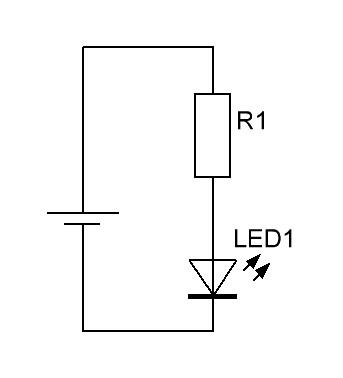
\includegraphics[width=\textwidth]{chapters/hardware-chapters/dc-led-resistor.jpg}
    \caption{Simplest way to power an LED.}
	\label{fig:dc-led-resistor}
  \end{minipage}
  \hfill
  \begin{minipage}[b]{0.65\textwidth}
    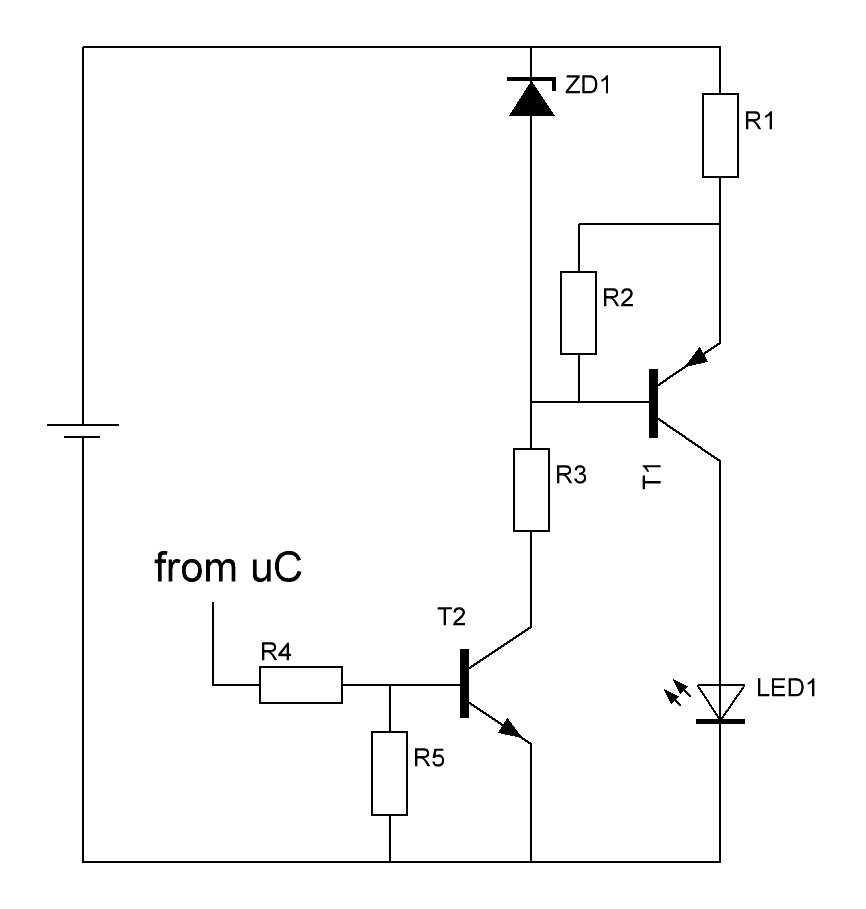
\includegraphics[width=\textwidth]{chapters/hardware-chapters/dc-led-current-source.jpg}
    \caption{Current source powering an LED.}
	\label{fig:dc-led-current-source}
  \end{minipage}
\end{figure}









\subsection{Current Sampler}

The most simple way to measure current in a DC environment is by using a series resistor.
The resistance does variate and therefor no noise is introduced in the sampled signal.
All the LEDs, and therefor all the current sources, are connected in parallel and a series resistor is connected in series with the LEDs and the power supply.
The voltage drop over the resistor is then linear proportional to the current that flows through it, according to Ohm's Law.
If the value of the resistor is chosen such that the maximum voltage will never exceed the rated voltage for a microprocessor, it can be directly measured by the microprocessor's ADC in question.









\subsection{Testbed}

To test the code sequences with actual hardware, a testbed was created.
The testbed works on DC and incorporates six individual controllable current sources that power strips of LEDs.
Each strip has six LEDs in series on them.
The current is measured by a series resistor en fed to the ADC of a microprocessor.
The entire schematic can be found in \autoref{app:dc-test-bed-schematic}. \todo{Transistor types}



The current sources and therefor the LEDs can be toggled on and off by a microprocessor.
By doing that the current that flows through the series resistor will change.
A change of voltage over the series resistor can then be measured by an ADC.


The Orthogonal and PN sequences, as discussed in \autoref{chp:cdma}, are zero and one valued.
These values can directly be used for the state of the LED.
The Orthogonal sequences will work, but only when the LEDs are synchronized with each other, due to the nature of these sequences (See \autoref{sec:orthogonal-sequences}.
However when using the Gold sequences, the LEDs can work without being synchronized with each other.
\todo{As shown in eval. raw incoming data of 6 Gold seq. and correlation with one or two ....}















